
\documentclass[runningheads]{llncs}
\usepackage[text={150mm,220mm},centering]{geometry}
\usepackage{graphicx}
\usepackage{float}
\usepackage{listings}

\begin{document}
\title{\large{Computational Intelligence Laboratory Exercise 2}}
\author{\large{Student Name: ChangXu \\ % Please write your name here
CCNU Student Number: 2019180034 \\ % Please write your CCNU student number here
UOW Student Number: 6643048}}  % Please write your UOW student number here


\authorrunning{CCNU Wollongong Joint Institute}
\institute{Central China Normal University Wollongong Joint Institute}

\maketitle


%-----------Please write your solutions to the questions in the assignment from here.---------------

\section{Problem 1 - Two Sprial Problem}
The 
problem 1 is Two Sprial Problem, 
it can be described as a two class problem
 where each class is an inter twined spiral on a two
dimensional plane. We can tell that this problem is a non-linear data problem. So I decide to use multi-neural network to solve this
problem.\\
With the codes in the other file, we get the result form different parameters:\\
\begin{figure}[H]
    \centering
    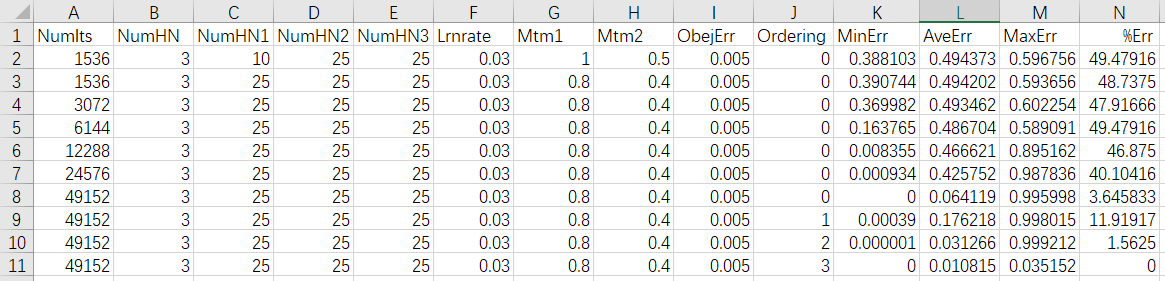
\includegraphics[scale=0.7]{data1.PNG}  
\end{figure}
So in this problem, when the number of iteration reach to more 
than 40000, the accurancy of prediction increase apparently. And
in training pattern, the Ordering 3 is selected each training
iteration perform better than the left way, which parameters is 
NumIts: 49152, NumHN: 3, NumHN1: 25, NumHN2: 25, NumHN3: 25. Lerning
rate is 0.03. The accurancy can reach 100\%.
Ordering 1 is the worst one in classify Two Sprial Problem. 

\section{Problem 2 – Abalone Age Problem }
Abalone Age Problem is to predict the age of abalone from physical measurements.
There are serveral points to determin the age such as sex, length, diameter,
height, whole weight, shucked weight, viscera weight, shell weight, And
rings. So the data should have 8 inputs in inputs layer.
\begin{figure}[H]
    \centering
    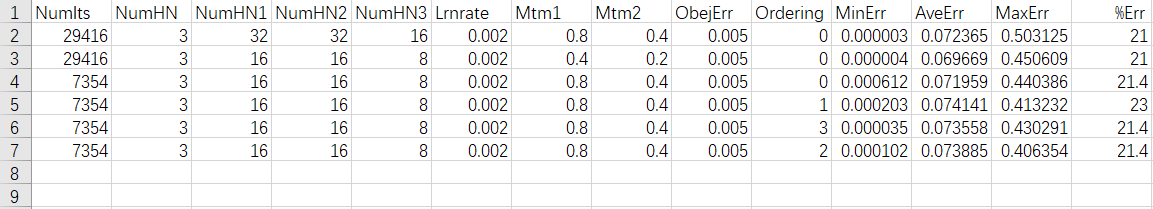
\includegraphics[scale=0.7]{data2.PNG}  
\end{figure}
\begin{figure}[H]
    \centering
    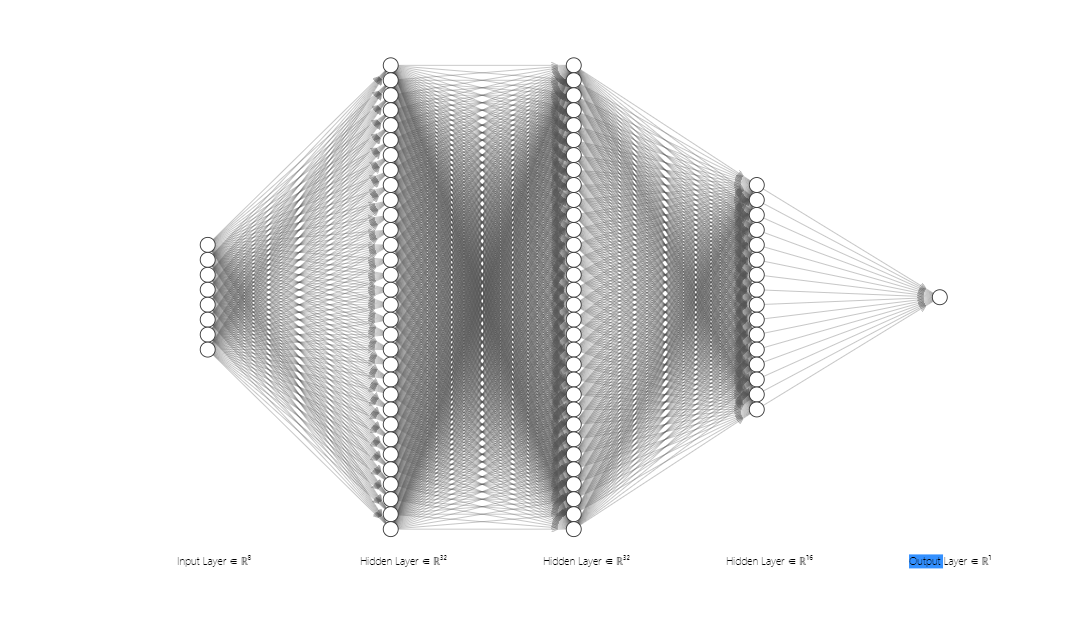
\includegraphics[scale=0.7]{MLP.PNG}  
\end{figure}

The same as problem 1, the ordering-1 has the worst perfomance the 
3 left training pattern. And the epoch number over 7354 will inflence
a little in the accurancy of prediction.The parameters of best perfomance
is NumIts: 7354, NumHN: 3, NumHN1: 16, NumHN2: 16, NumHN3: 8. Lerning
rate is 0.03. The accurancy can reach 80\%.
\section{ SPECT Heart Diagnosis Problem }
A SPECT scan of the heart is a noninvasive nuclear imaging test.
It uses radioactive tracers that are injected into the blood to
produce pictures of your heart. Doctors use SPECT to diagnose 
coronary artery disease and find out if a heart attack has 
occurred. We need to know whether the people is normal or abnormal
catagoried into 0 and 1. The data set extract 44 features to training
this calssification modle. From the MLP algorithm:
\begin{figure}[H]
    \centering
    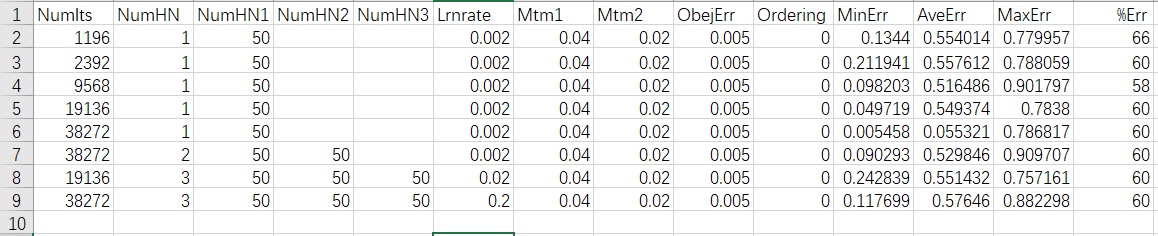
\includegraphics[scale=0.7]{data3.PNG}  
\end{figure}
We can know from the blank, the accurancy does not change
ignoring how the parameters has changed. The MLP might not
suit this problem.
\end{document}
